\section{Experimental Evaluation - Tracking}

\begin{frame}
	\frametitle{Evaluating a Tracking Algorithm}
	
	\Large
	
	\vspace{0.45cm}
	
	The CLEAR MOT (Kasturi et al. \cite{Kasturi09}) metrics \emph{MOTA} and \emph{MOTP} are the
	de-facto standard for evaluating a tracking method:
	
	\vspace{-0.5cm}
	
	\begin{equation*}
		MOTA = 1 - \frac{\sum_{t=1}^{N_{frames}} \big [ c_m(m_t) + c_f(fp_t) + cs(ID\mbox{-}S_t) \big ]}{\sum_{t=1}^{N_{frames}} N_G^{(t)}}
	\end{equation*}
	
	\vspace{0.4cm}
	
	\begin{equation*}
		MOTP = \frac{\sum_{i=1}^{N_{mapped}} \sum_{t=1}^{N_{frames}^{(t)}} \Big [ \frac{| G_i^{(t)} \cap D_i^{(t)} |}{| G_i^{(t)} \cup D_i^{(t)} |} \Big ] }{\sum_{t=1}^{N_{frames}} N_{mapped}^{(t)}}
	\end{equation*}
	
	\vspace{0.3cm}
	
	\tiny
	
	\cite{Kasturi09} R. Kasturi \emph{et al.},  ``Framework for performance evaluation of face, text,
	and vehicle detection and tracking in video: data,\\ \hspace{0.25cm} metrics, and protocol'', PAMI,
	2009 \\
\end{frame}

\begin{frame}
	\frametitle{Experimental Evaluation}
	\framesubtitle{Single-Sensor, Multi-Object}
	
	\large
	
	\begin{columns}[t]
		\only<1->
		{
			\column{0.8\textwidth}
			
			\begin{block}{Boat Visual Tracking}
				automatic surveillance system in the maritime domain
			\end{block}
			
			\column{0.15\textwidth}
		}
	\end{columns}
	
	\vspace{0.3cm}
	
	\begin{center}
		\begin{tikzpicture}
			\node at (0,0) [draw=black,ultra thick,inner sep=0pt]  {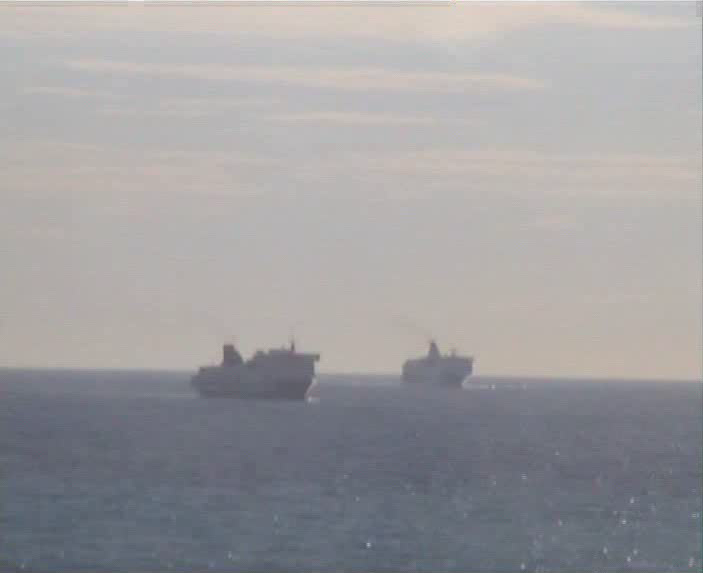
\includegraphics[height=3.1cm]{Figures/Boat-1}};
			\node at (3.95,0) [draw=black,ultra thick,inner sep=0pt]  {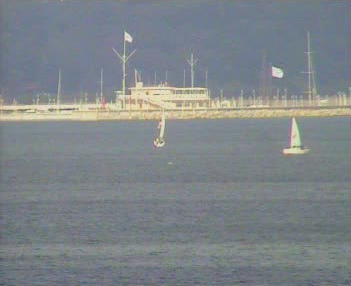
\includegraphics[height=3.1cm]{Figures/Boat-2}};
			\node at (7.95,0) [draw=black,ultra thick,inner sep=0pt]  {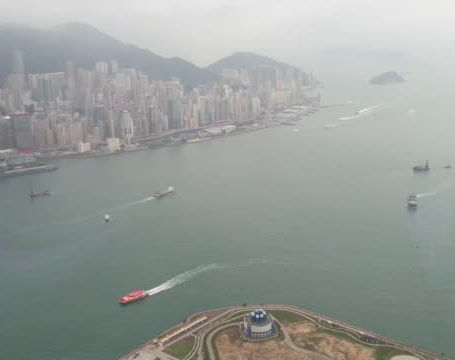
\includegraphics[height=3.1cm]{Figures/Boat-3}};
		\end{tikzpicture}
	\end{center}
	
	\vspace{0.45cm}
	
	\tiny
	
	\textbf{Enhancing Automatic Maritime Surveillance Systems with Visual Information} \\
	D. D. Bloisi, F. Previtali, A. Pennisi, D. Nardi, M. Fiorini \\
	\emph{IEEE Transaction on Intelligent Transportation Systems} [second revision] \\
\end{frame}

\begin{frame}
	\frametitle{Quantitative Evaluation}
	\framesubtitle{Maritime Domain}
	
	\large
	
	\begin{table}[!t]
		\renewcommand{\arraystretch}{1.3}
		\caption{\large Tracking performance on the maritime domain. MOTA (higher the better) considers
				 the number of missed detections, the number of false positives and the switches of
				 identities. MOTP (higher the better) considers the precision of the detections.}
		\centering
		\vspace{0.2cm}
		
		\begin{tabular}{ccc}
			\hline
			\hline
			\textbf{Video} & \textbf{MOTA} & \textbf{MOTP} \\
			\hline
			occlusions-1.avi & 0.815 & 0.613 \\
			\hline
			occlusions-2.avi & 0.910 & 0.554 \\
			\hline
			high-view.avi & 0.910 & 0.604 \\
			\hline
		\hline
		\end{tabular}
	\end{table}
\end{frame}

\begin{frame}
	\frametitle{Qualitative Evaluation}
	\framesubtitle{Maritime Domain - Blue Water}
	
	\begin{center}
		\href{run:../Scripts/boat-1.sh}
		{
			\begin{tikzpicture}
				\node at (0,0) [draw=black,ultra thick,inner sep=0pt]
				{
					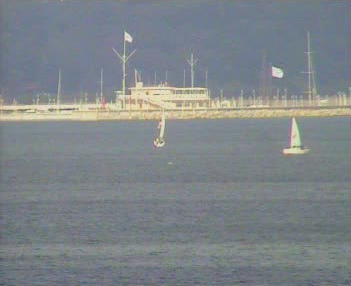
\includegraphics[width=0.65\linewidth]{Figures/Boat-2.png}
				};
			\end{tikzpicture}
		}
	\end{center}
\end{frame}

\begin{frame}
	\frametitle{Qualitative Evaluation}
	\framesubtitle{Maritime Domain - Hong Kong Port}
	
	\begin{center}
		\href{run:../Scripts/boat-2.sh}
		{
			\begin{tikzpicture}
				\node at (0,0) [draw=black,ultra thick,inner sep=0pt]
				{
					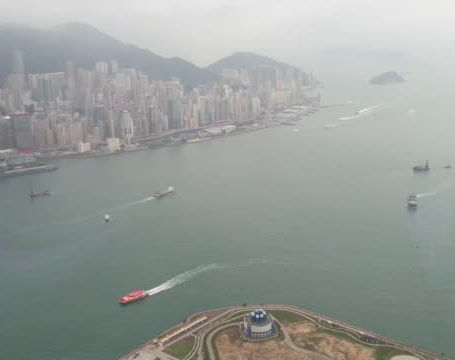
\includegraphics[width=0.65\linewidth]{Figures/Boat-3.png}
				};
			\end{tikzpicture}
		}
	\end{center}
\end{frame}

\begin{frame}
	\frametitle{Experimental Evaluation}
	\framesubtitle{Multi-Sensor, Single-Object}
	
	\large
	
	\vspace{-0.3cm}
	
	\begin{columns}[t]
		\only<1->
		{
			\column{0.8\textwidth}
			
			\begin{block}{Soccer Robots}
				used to solve the localisation field symmetry problem
			\end{block}
			
			\column{0.15\textwidth}
		}
	\end{columns}
	
	\vspace{0.15cm}
	
	\begin{center}
		\begin{tikzpicture}
			\node at (0,0) [draw=black,ultra thick,inner sep=0pt]
			{
				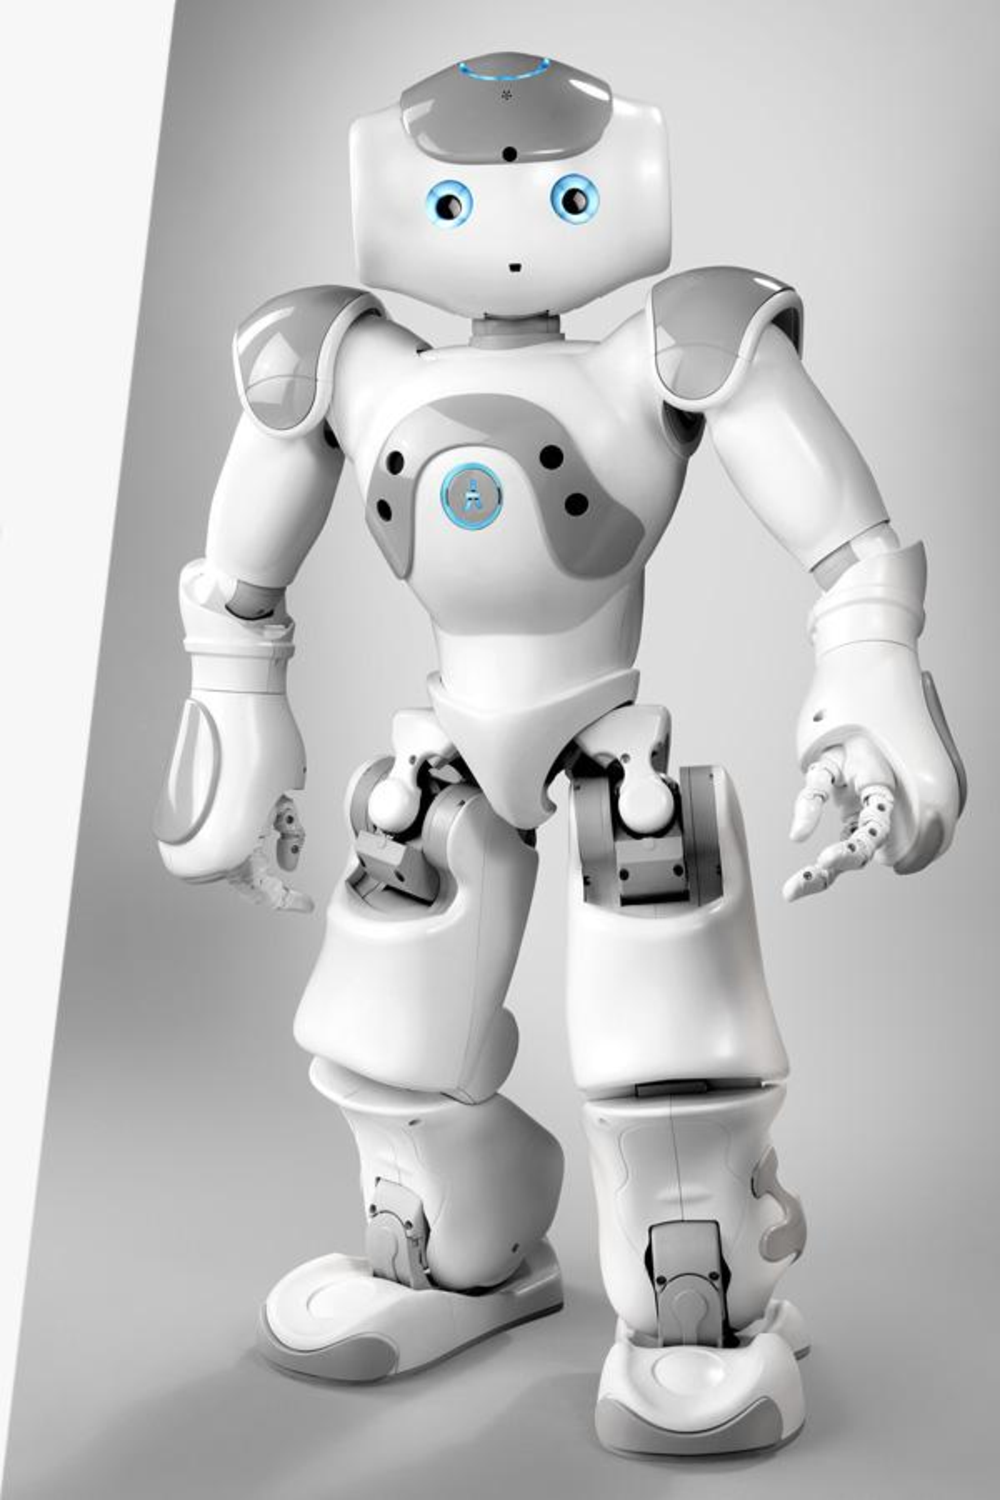
\includegraphics[scale=0.2]{Figures/Nao}
			};
		\end{tikzpicture}
	\end{center}
	
	\tiny
	
	\textbf{Disambiguating Localization Symmetry through a Multi-Clustered Particle Filtering} \\
	F. Previtali, G. Gemignani, L. Iocchi, D. Nardi \\
	\emph{IEEE International Conference on Multisensor Fusion and Integration for Intelligent Systems,
	2015} \\
\end{frame}

\begin{frame}
	\frametitle{Challenge}
	
	\Large
	
	\vspace{0.25cm}
	
	\begin{figure}
		\centering
		\begin{tikzpicture}
			\node at (0,0) [draw=white,ultra thick,inner sep=0pt]
			{
				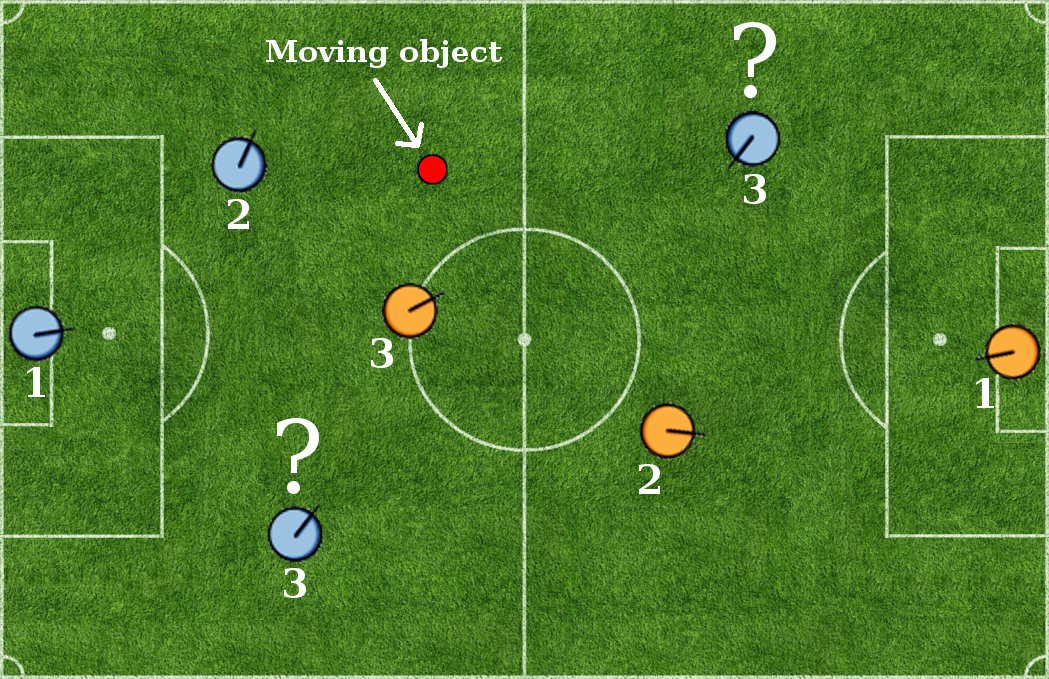
\includegraphics[width=0.8\linewidth]{Figures/Challenge}
			};
		\end{tikzpicture}
	\end{figure}
	
	\vspace{-0.4cm}
	
	\begin{center}
		What is the real position of the blue robot number 3?
	\end{center}
\end{frame}

\begin{frame}
	\frametitle{Quantitative Evaluation}
	\framesubtitle{RoboCup Domain}
	
	\large
	
	\vspace{-0.85cm}
	
	Simulating 3 Aldebaran Nao robots playing soccer, one of them alternatively forced to be inversely
	localised
	
	\Large
	
	\vspace{-0.6cm}
	
	\begin{columns}[T]
		\column{1.02\textwidth}
		
	\begin{figure}
		\centering
		
		\begin{tikzpicture}
			\node at (0,0) [draw=white,ultra thick,inner sep=0pt]
			{
				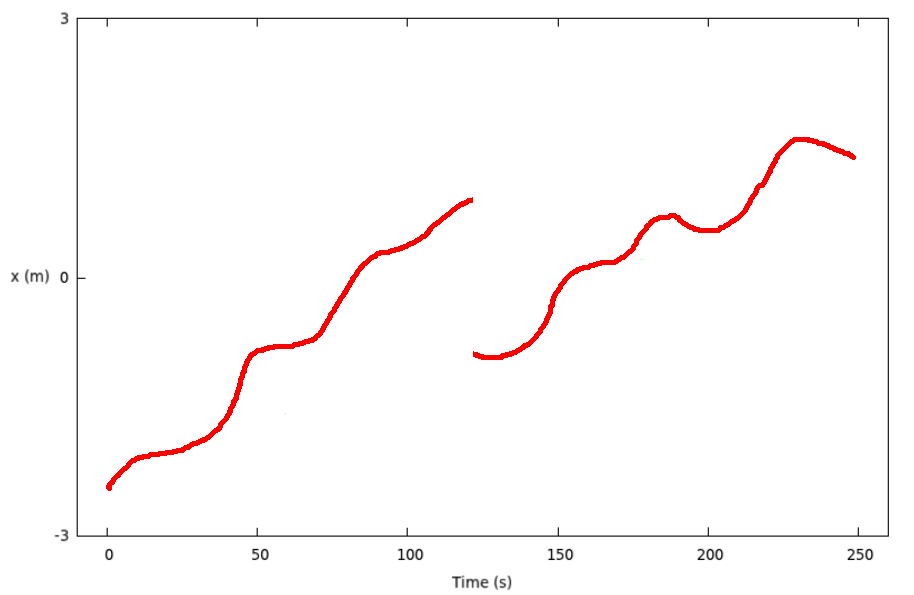
\includegraphics[width=0.34\linewidth]{Figures/Result-Scenario-2_Robot-1}
			};
			\node at (4.1,0) [draw=white,ultra thick,inner sep=0pt]
			{
				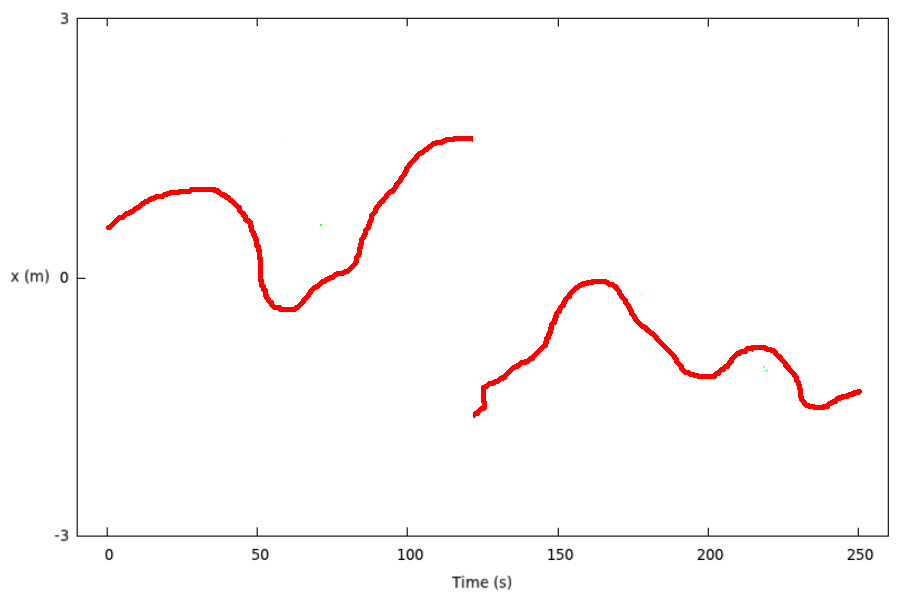
\includegraphics[width=0.34\linewidth]{Figures/Result-Scenario-2_Robot-2}
			};
			\node at (0,-2.9) [draw=white,ultra thick,inner sep=0pt]
			{
				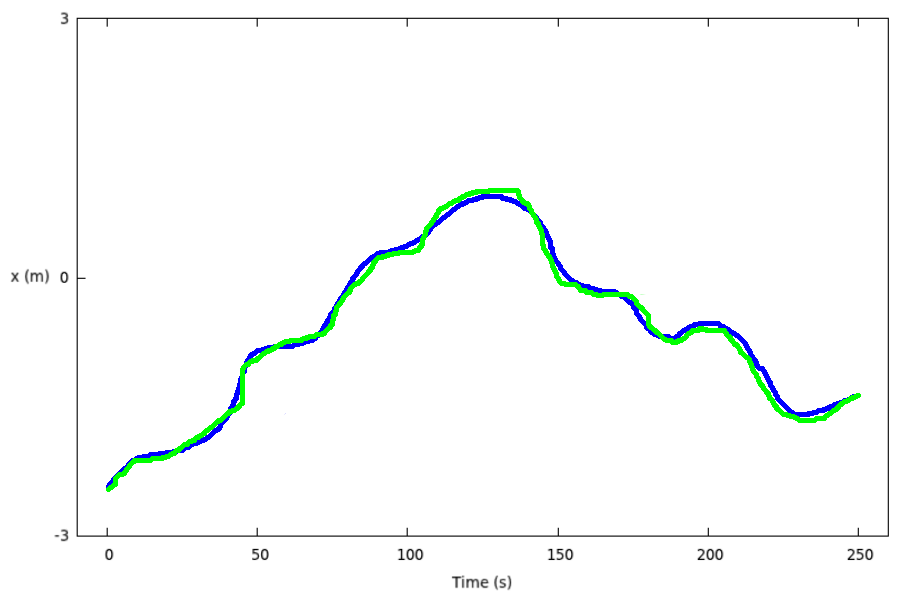
\includegraphics[width=0.34\linewidth]{Figures/Result-Scenario-2_Robot-1-GT}
			};
			\node at (4.1,-2.9) [draw=white,ultra thick,inner sep=0pt]
			{
				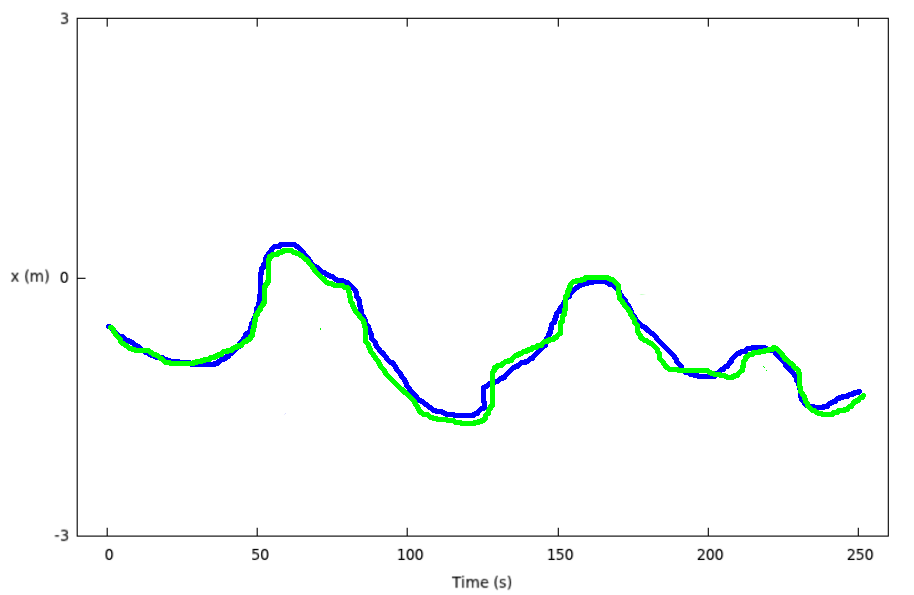
\includegraphics[width=0.34\linewidth]{Figures/Result-Scenario-2_Robot-2-GT}
			};
			\node at (8.2,0) [draw=white,ultra thick,inner sep=0pt]
			{
				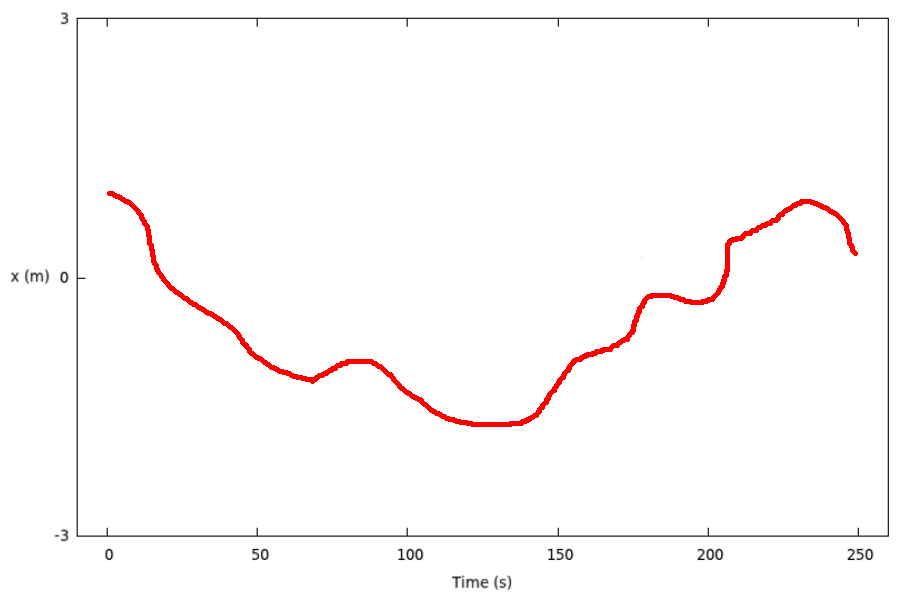
\includegraphics[width=0.34\linewidth]{Figures/Result-Scenario-2_Robot-3}
			};
			\node at (8.2,-2.9) [draw=white,ultra thick,inner sep=0pt]
			{
				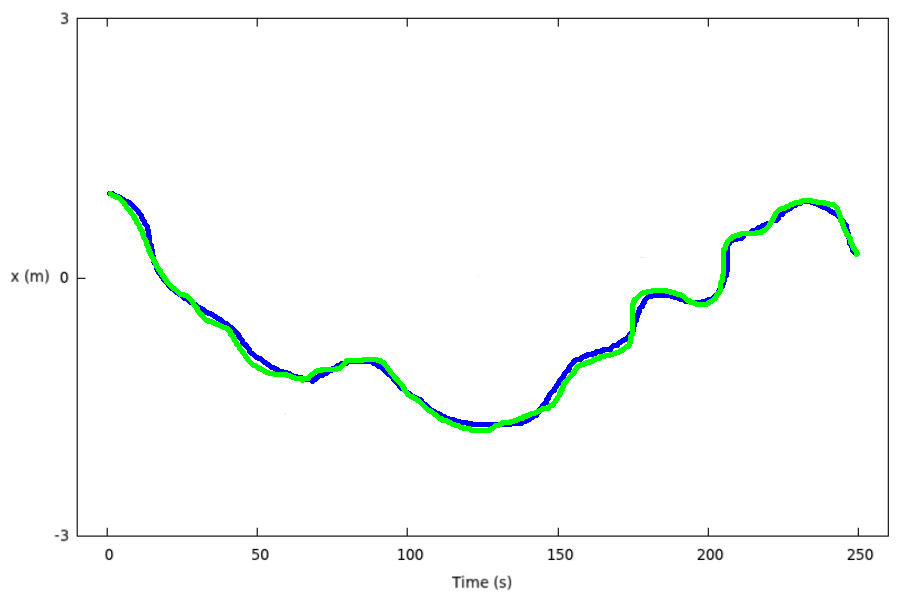
\includegraphics[width=0.34\linewidth]{Figures/Result-Scenario-2_Robot-3-GT}
			};
		\end{tikzpicture}
	\end{figure}
	\end{columns}
	
	\vspace{-6.15cm}
	
	\begin{tabbing}
		\hspace{0.21cm}
		\tiny
		\textbf{Robot 1 - Localization}
		\hspace{1.79cm}
		\textbf{Robot 2 - Localization}
		\hspace{1.79cm}
		\textbf{Robot 3 - Localization}
	\end{tabbing}
	
	\vspace{-1cm}
	
	\begin{tabbing}
		\hspace{0.4cm}
		\tiny
		\textcolor{blue}{Correctly}
	\end{tabbing}
	
	\vspace{-1.2cm}
	
	\begin{tabbing}
		\hspace{0.42cm}
		\tiny
		\textcolor{blue}{localized}
	\end{tabbing}
	
	\vspace{-1.17cm}
	
	\begin{tabbing}
		\footnotesize
		\hspace{0.87cm}
		\textcolor{blue}{$ \searrow $}
	\end{tabbing}
	
	\vspace{-1.43cm}
	
	\begin{tabbing}
		\footnotesize
		\hspace{2.68cm}
		\textcolor{blue}{$ \nwarrow $}
	\end{tabbing}
	
	\vspace{-1.2cm}
	
	\begin{tabbing}
		\hspace{2.53cm}
		\tiny
		\textcolor{blue}{Wrongly}
	\end{tabbing}
	
	\vspace{-1.2cm}
	
	\begin{tabbing}
		\hspace{2.52cm}
		\tiny
		\textcolor{blue}{localized}
	\end{tabbing}
	
	\vspace{-1.83cm}
	
	\begin{tabbing}
		\footnotesize
		\hspace{4.8cm}
		\textcolor{blue}{$ \nearrow $}
	\end{tabbing}
	
	\vspace{-1.2cm}
	
	\begin{tabbing}
		\hspace{4.35cm}
		\tiny
		\textcolor{blue}{Wrongly}
	\end{tabbing}
	
	\vspace{-1.2cm}
	
	\begin{tabbing}
		\hspace{4.34cm}
		\tiny
		\textcolor{blue}{localized}
	\end{tabbing}
	
	\vspace{-2.75cm}
	
	\begin{tabbing}
		\hspace{6.82cm}
		\tiny
		\textcolor{blue}{Correctly}
	\end{tabbing}
	
	\vspace{-1.2cm}
	
	\begin{tabbing}
		\hspace{6.84cm}
		\tiny
		\textcolor{blue}{localized}
	\end{tabbing}
	
	\vspace{-1.17cm}
	
	\begin{tabbing}
		\footnotesize
		\hspace{7cm}
		\textcolor{blue}{$ \swarrow $}
	\end{tabbing}
	
	\vspace{-1.79cm}
	
	\begin{tabbing}
		\hspace{9.52cm}
		\tiny
		\textcolor{blue}{Correctly}
	\end{tabbing}
	
	\vspace{-1.2cm}
	
	\begin{tabbing}
		\hspace{9.54cm}
		\tiny
		\textcolor{blue}{localized}
	\end{tabbing}
	
	\vspace{-1.17cm}
	
	\begin{tabbing}
		\footnotesize
		\hspace{9.99cm}
		\textcolor{blue}{$ \searrow $}
	\end{tabbing}
	
	\vspace{0.01cm}
	
	\begin{tabbing}
		\hspace{0.21cm}
		\tiny
		\textbf{Robot 1 - Filtered vs Ground-Truth}
		\hspace{0.53cm}
		\textbf{Robot 2 - Filtered vs Ground-Truth}
		\hspace{0.53cm}
		\textbf{Robot 3 - Filtered vs Ground-Truth}
	\end{tabbing}
\end{frame}

\begin{frame}
	\frametitle{Qualitative Evaluation}
	\framesubtitle{RoboCup Iran Open}
	
	\begin{center}
		\href{run:../Scripts/nao.sh}
		{
			\begin{tikzpicture}
				\node at (0,0) [draw=black,ultra thick,inner sep=0pt]
				{
					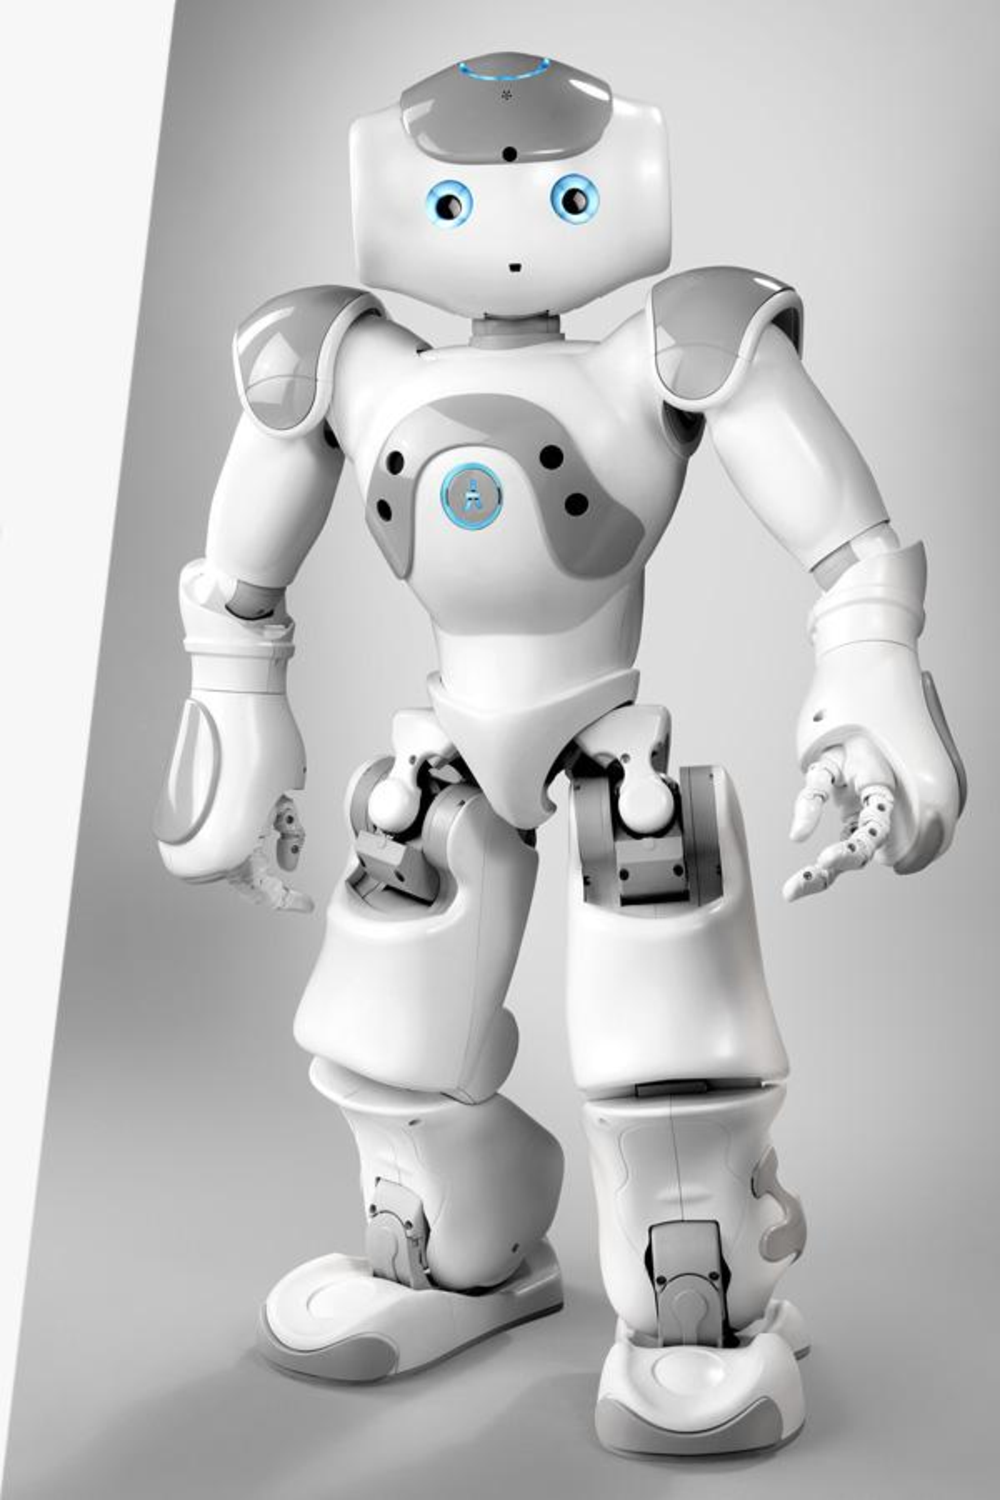
\includegraphics[width=0.9\linewidth]{Figures/Nao}
				};
			\end{tikzpicture}
		}
	\end{center}
\end{frame}

\begin{frame}
	\frametitle{Experimental Evaluation}
	\framesubtitle{Multi-Sensor, Multi-Object}
	
	\large
	
	\vspace{-0.35cm}
	
	\begin{columns}[t]
		\only<1->
		{
			\column{0.8\textwidth}
			
			\begin{block}{Issia Soccer}
				tracking of players in a real soccer match
			\end{block}
			
			\column{0.15\textwidth}
		}
	\end{columns}
	
	\begin{center}
		\begin{tikzpicture}
			\node at (2.39,0) [draw=black,ultra thick,inner sep=0pt]  {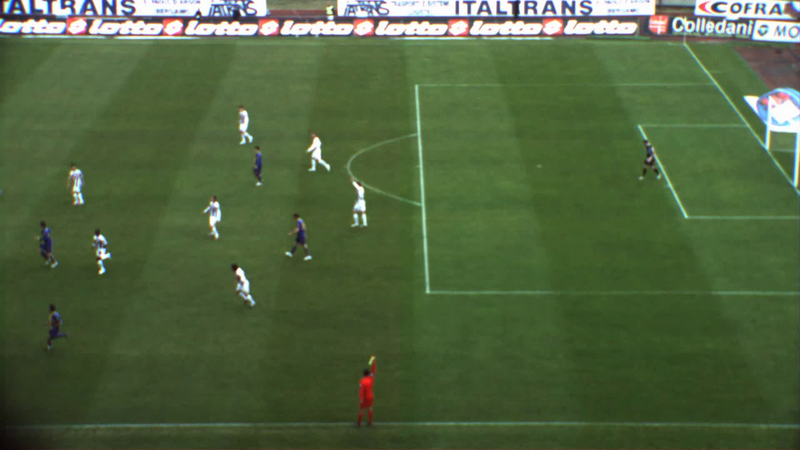
\includegraphics[height=2.1cm]{Figures/IssiaSoccer-Camera1}};
			\node at (6.26,0) [draw=black,ultra thick,inner sep=0pt]  {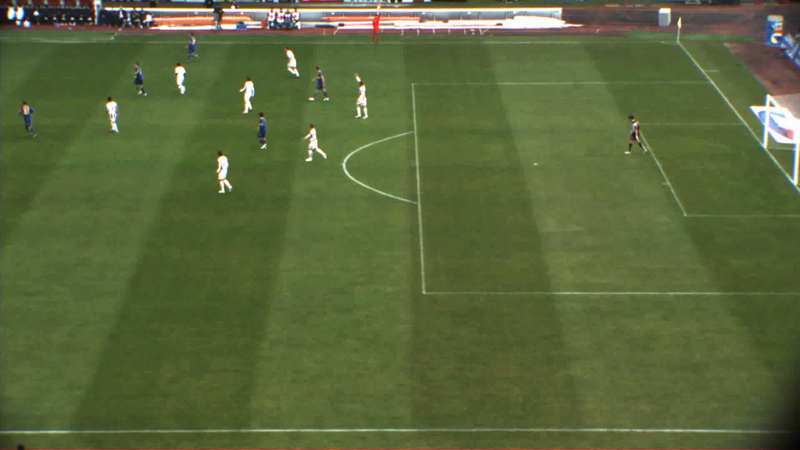
\includegraphics[height=2.1cm]{Figures/IssiaSoccer-Camera2}};
			\node at (2.39,-2.22) [draw=black,ultra thick,inner sep=0pt]  {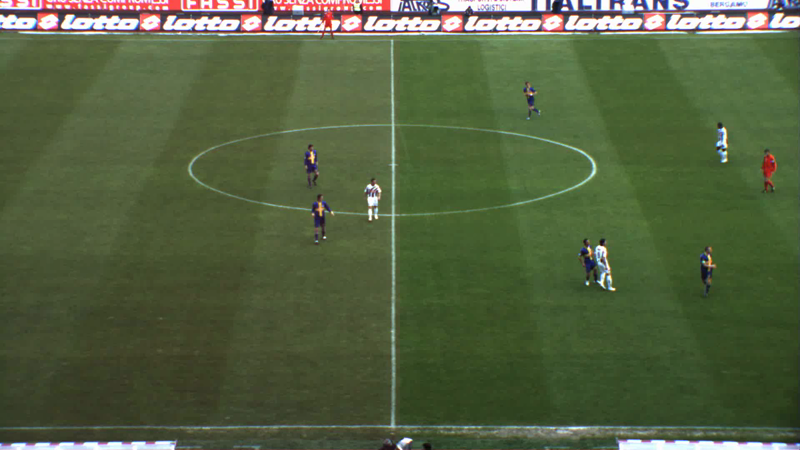
\includegraphics[height=2.1cm]{Figures/IssiaSoccer-Camera3}};
			\node at (6.26,-2.22) [draw=black,ultra thick,inner sep=0pt]  {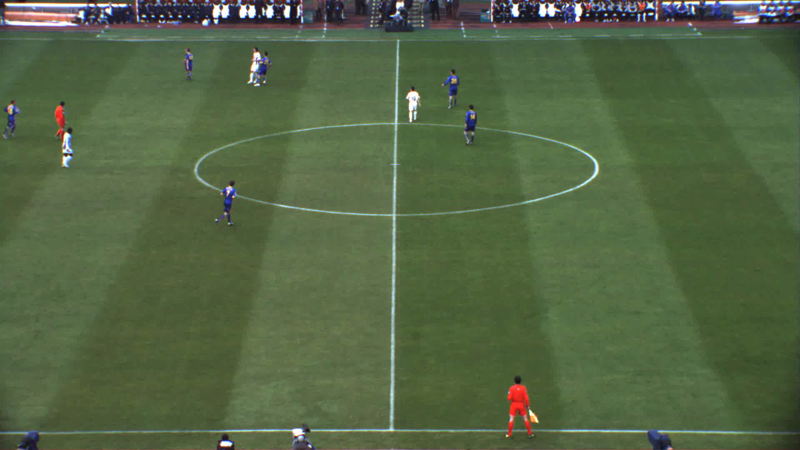
\includegraphics[height=2.1cm]{Figures/IssiaSoccer-Camera4}};
		\end{tikzpicture}
	\end{center}
	
	\vspace{-0.05cm}
	
	\tiny
	
	\textbf{A Distributed Approach for Real-Time Multi-Camera Multi-Object Tracking} \\
	F. Previtali, D. D. Bloisi, L. Iocchi \\
	\emph{Journal on Computer Vision and Image Understanding} [second revision] \\
\end{frame}

\begin{frame}
	\frametitle{Quantitative Evaluation}
	\framesubtitle{People Domain - Issia Soccer}
	
	\Large
	
	\begin{table}[!t]
		\renewcommand{\arraystretch}{1.3}
		\centering
		\begin{tabular}{lcccc}
			\hline
			\hline
			\multicolumn{1}{c}{\begin{tabular}[c]{@{}c@{}}\textbf{Method} \end{tabular}} & \textbf{MOTA} & \textbf{MOTP} \\
			\hline
			PTracking - Camera 1 & 0.723 & 0.612 \\
			\hline
			PTracking - Camera 1, 2 & 0.789 & 0.638 \\
			\hline
			PTracking - Camera 1, 2, 3 & 0.817 & 0.651 \\
			\hline
			PTracking - Camera 1, 2, 3, 4 & 0.894 & 0.706 \\
			\hline
		\hline
		\end{tabular}
	\end{table}
\end{frame}

\begin{frame}
	\frametitle{Qualitative Evaluation}
	\framesubtitle{People Domain - Issia Soccer}
	
	\begin{center}
		\href{run:../Scripts/issia.sh}
		{
			\begin{tikzpicture}
				\node at (0,0) [draw=black,ultra thick,inner sep=0pt]
				{
					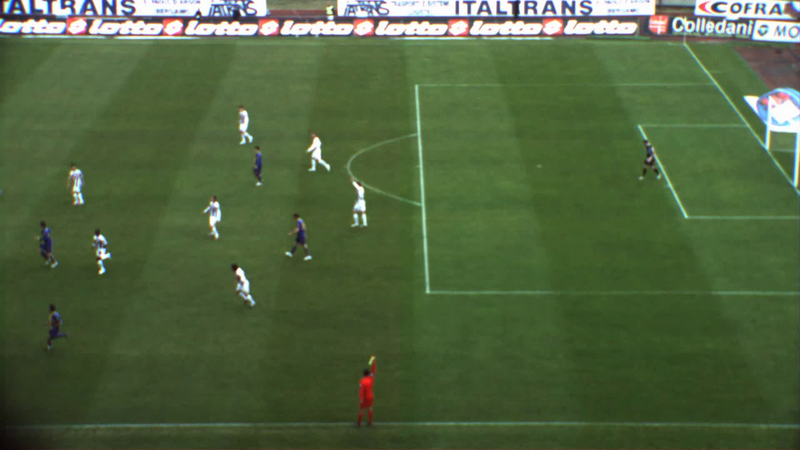
\includegraphics[width=0.9\linewidth]{Figures/IssiaSoccer-Camera1}
				};
			\end{tikzpicture}
		}
	\end{center}
\end{frame}

\begin{frame}
	\frametitle{Experimental Evaluation}
	\framesubtitle{Multi-Sensor, Multi-Object}
	
	\large
	
	\vspace{-0.45cm}
	
	\begin{columns}[t]
		\only<1->
		{
			\column{0.8\textwidth}
			
			\begin{block}{PETS-2009}
				tracking of individuals within a crowd
			\end{block}
			
			\column{0.15\textwidth}
		}
	\end{columns}
	
	\vspace{0.1cm}
	
	\begin{center}
		\begin{tikzpicture}
			\node at (0,0) [draw=black,ultra thick,inner sep=0pt]  {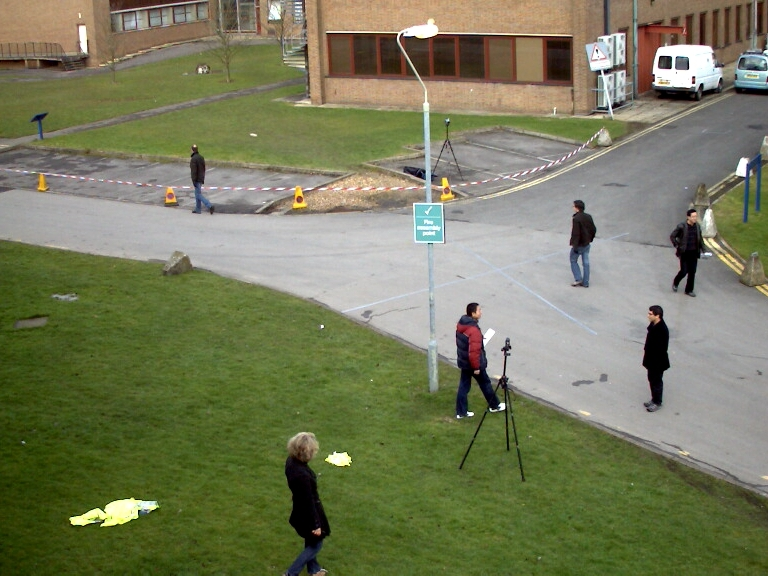
\includegraphics[height=2.55cm]{Figures/PETS2009-1}};
			\node at (3.55,0) [draw=black,ultra thick,inner sep=0pt]  {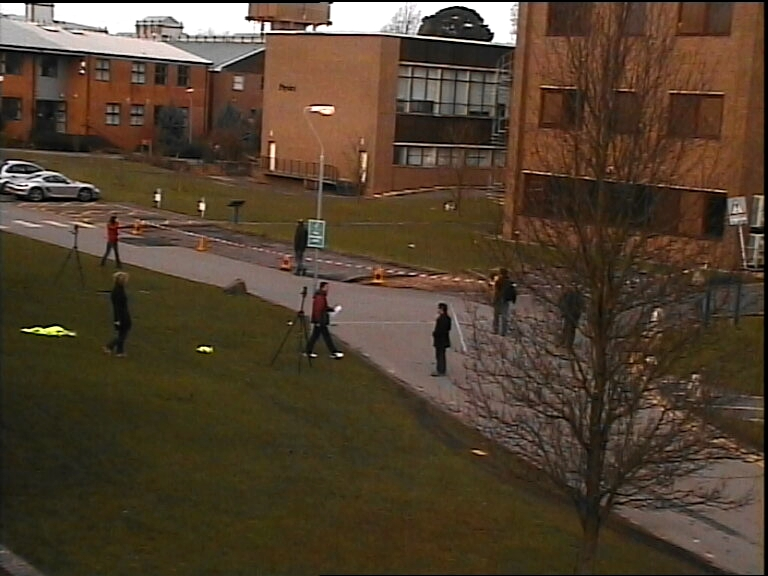
\includegraphics[height=2.55cm]{Figures/PETS2009-3}};
			\node at (7.17,0) [draw=black,ultra thick,inner sep=0pt]  {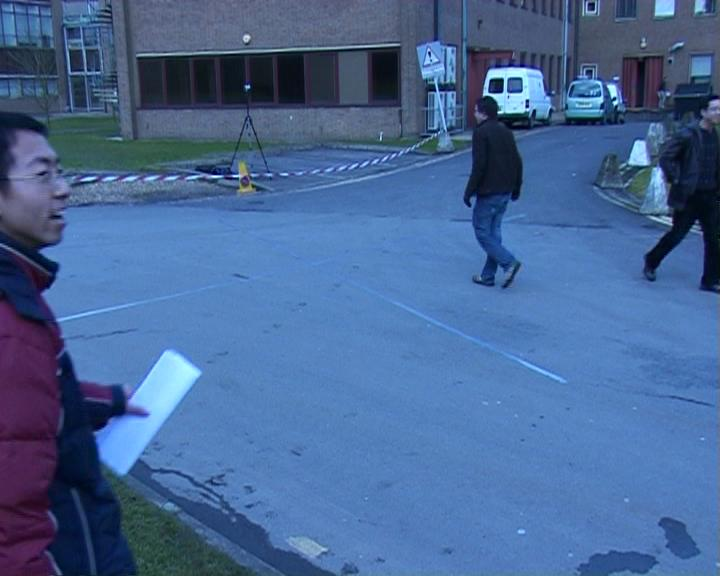
\includegraphics[height=2.55cm]{Figures/PETS2009-6}};
			\node at (1.8,-2.7) [draw=black,ultra thick,inner sep=0pt]  {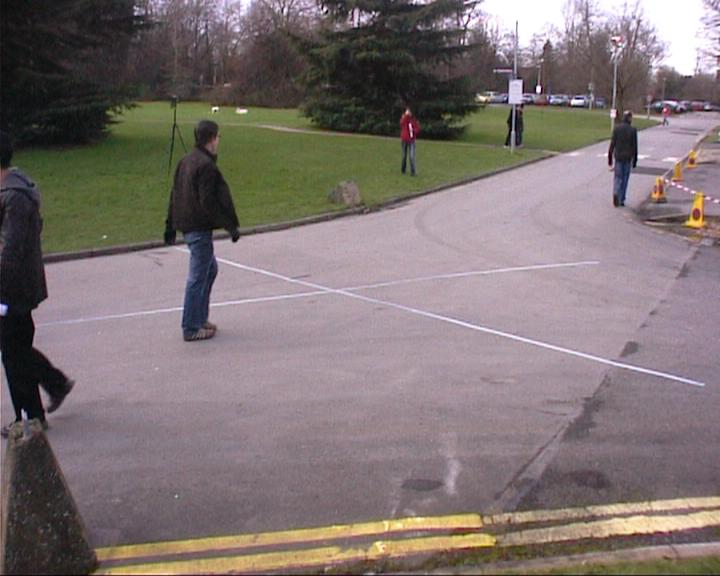
\includegraphics[height=2.55cm]{Figures/PETS2009-7}};
			\node at (5.5,-2.7) [draw=black,ultra thick,inner sep=0pt]  {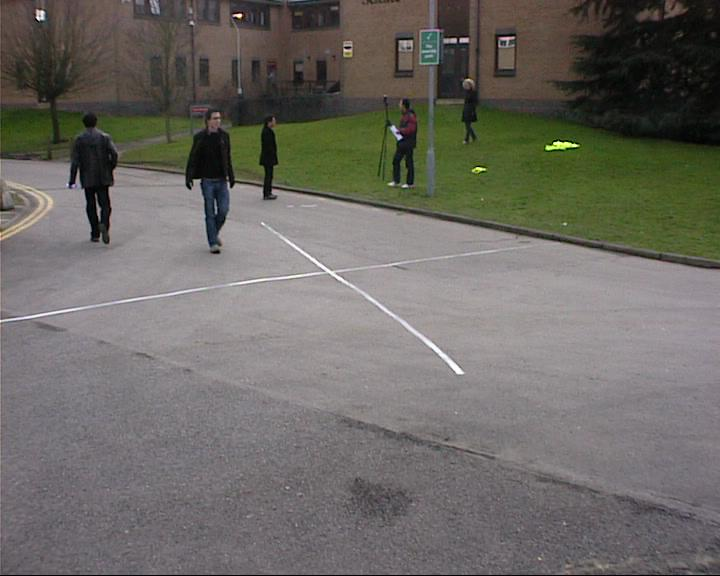
\includegraphics[height=2.55cm]{Figures/PETS2009-8}};
		\end{tikzpicture}
	\end{center}
\end{frame}

\begin{frame}
	\frametitle{Quantitative Evaluation}
	\framesubtitle{People Domain - PETS-2009}
	
	\large
	
	\begin{table}[!t]
		\renewcommand{\arraystretch}{1.3}
		\centering
		\begin{tabular}{ccccc}
			\hline
			\hline
			\textbf{Method} & \textbf{MOTA} & \textbf{MOTP} & \textbf{Type} & \textbf{Real-Time} \\
			\hline
			Leal-Taix\'{e} \cite{Leal11} & 0.67 & 0.534 & OFFLINE & NO \\
			\hline
			Berclaz \cite{Berclaz11} & 0.732 & 0.603 & OFFLINE & NO \\
			\hline
			Henriques \cite{Henriques11} & 0.833 & 0.711 & OFFLINE & NO \\
			\hline
			Breitenstein \cite{Breitenstein11} & 0.745 & 0.563 & ONLINE & NO \\
			\hline
			Yang \cite{Yang09} & 0.759 & 0.538 & ONLINE & NO \\
			\hline
			Bae \cite{Bae14} & 0.830 & 0.696 & ONLINE & \textbf{YES} \\
			\hline
			PTracking & \textbf{0.874} & \textbf{0.722} & ONLINE & \textbf{YES (30.2 FPS)} \\
			\hline
			PTracking$^*$ & \textbf{0.882} & \textbf{0.717} & ONLINE & NO (11.8 FPS) \\
			\hline
		\hline
		\end{tabular}
	\end{table}
\end{frame}

\begin{frame}
	\frametitle{Experimental Evaluation}
	\framesubtitle{Multi-Sensor, Multi-Object}
	
	\large
	
	\begin{columns}[t]
		\only<1->
		{
			\column{0.8\textwidth}
			
			\begin{block}{Prey-Predator Game}
				demonstrating the advantages of using mobile sensors
			\end{block}
			
			\column{0.15\textwidth}
		}
	\end{columns}
	
	\vspace{0.1cm}
	
	\begin{center}
		\begin{tikzpicture}
			\node at (0,0) [draw=black,ultra thick,inner sep=0pt]  {\includegraphics[height=3.25cm]{Figures/Map-1_}};
			\node at (6,0) [draw=black,ultra thick,inner sep=0pt]  {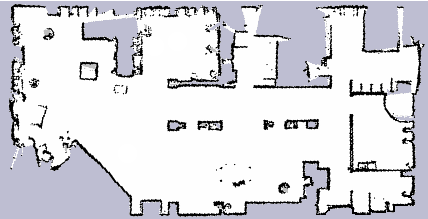
\includegraphics[height=3.25cm]{Figures/Map-2_}};
		\end{tikzpicture}
	\end{center}
	
	\vspace{0.52cm}
	
	\tiny
	
	\textbf{PTracking: Distributed Multi-Agent Multi-Object Tracking through Multi-Clustered Particle
	Filtering} \\
	F. Previtali, L. Iocchi \\
	\emph{IEEE International Conference on Multisensor Fusion and Integration for Intelligent Systems,
	2015} \\
\end{frame}

\begin{frame}
	\frametitle{Quantitative Evaluation}
	\framesubtitle{DIAG}
	
	\small
	
	\begin{table}[!t]
		\centering
		\begin{tabular}{ccccc}
			\cline{1-5}
			\multicolumn{1}{l}{} & \multicolumn{4}{c}{\textbf{\begin{tabular}[c]{@{}c@{}}
			Prey-Predator Distance (avg $ \pm $ std. dev.)\end{tabular}}} \\ \hline
			\multicolumn{1}{c}{\textbf{\#}} & \textbf{Setting 1} & \textbf{Setting 2} &
			\textbf{Setting 3} & \textbf{Setting 4} \\
			
			\multicolumn{1}{c}{1} & 3.04 $ \pm $ 0.63 $ m $ & 2.70 $ \pm $ 0.49
								  $ m $ & 2.02 $ \pm $ 0.38 $ m $ & 1.12 $ \pm $
								  0.19 $ m $ \\
			\multicolumn{1}{c}{2} & 2.95 $ \pm $ 0.80 $ m $ & 2.65 $ \pm $ 0.48
								  $ m $ & 1.95 $ \pm $ 0.42 $ m $ & 1.15 $ \pm $
								  0.20 $ m $ \\
			\multicolumn{1}{c}{3} & 3.12 $ \pm $ 0.53 $ m $ & 2.87 $ \pm $ 0.56
								  $ m $ & 2.03 $ \pm $ 0.41 $ m $ & 1.13 $ \pm $
								  0.19 $ m $ \\
			\multicolumn{1}{c}{4} & 3.01 $ \pm $ 0.69 $ m $ & 2.73 $ \pm $ 0.49
								  $ m $ & 2.06 $ \pm $ 0.38 $ m $ & 1.08 $ \pm $
								  0.22 $ m $ \\
			\multicolumn{1}{c}{5} & 2.99 $ \pm $ 0.72 $ m $ & 2.86 $ \pm $ 0.61
								  $ m $ & 1.99 $ \pm $ 0.40 $ m $ & 1.11 $ \pm $
								  0.17 $ m $ \\
			\hline
			
			\\
			
			\hline
			\multicolumn{1}{l}{} & \multicolumn{4}{c}{\textbf{\begin{tabular}[c]
			{@{}c@{}}Tracking Performance (MOTA,MOTP)\end{tabular}}} \\ \hline
			\multicolumn{1}{c}{\textbf{\#}} & \textbf{Setting 1} & \textbf{Setting 2} &
			\textbf{Setting 3} & \textbf{Setting 4} \\
			
			\multicolumn{1}{c}{1} & (0.63,0.45) & (0.67,0.49) & (0.75,0.51) & (0.94,0.75) \\
			\multicolumn{1}{c}{2} & (0.59,0.42) & (0.65,0.45) & (0.73,0.49) & (0.92,0.74) \\
			\multicolumn{1}{c}{3} & (0.64,0.41) & (0.69,0.48) & (0.70,0.47) & (0.95,0.77) \\
			\multicolumn{1}{c}{4} & (0.62,0.45) & (0.62,0.40) & (0.74,0.50) & (0.92,0.75) \\
			\multicolumn{1}{c}{5} & (0.57,0.39) & (0.64,0.44) & (0.70,0.48) & (0.94,0.77) \\
			\hline
		\end{tabular}
	\end{table}
\end{frame}

\begin{frame}
	\frametitle{Quantitative Evaluation}
	\framesubtitle{Peccioli House}
	
	\small
	
	\begin{table}
		\centering
		\begin{tabular}{ccccc}
			\cline{1-5}
			\multicolumn{1}{l}{} & \multicolumn{4}{c}{\textbf{\begin{tabular}[c]{@{}c@{}}
			Prey-Predator Distance (avg $ \pm $ std. dev.)\end{tabular}}} \\ \hline
			\multicolumn{1}{c}{\textbf{\#}} & \textbf{Setting 1} & \textbf{Setting 2} &
			\textbf{Setting 3} & \textbf{Setting 4} \\
			
			\multicolumn{1}{c}{1} & 2.84 $ \pm $ 0.59 $ m $ & 2.55 $ \pm $ 0.47
								  $ m $ & 1.85 $ \pm $ 0.38 $ m $ & 1.07 $ \pm $
								  0.18 $ m $ \\
			\multicolumn{1}{c}{2} & 2.85 $ \pm $ 0.74 $ m $ & 2.52 $ \pm $ 0.51
								  $ m $ & 1.84 $ \pm $ 0.40 $ m $ & 1.05 $ \pm $
								  0.21 $ m $ \\
			\multicolumn{1}{c}{3} & 3.03 $ \pm $ 0.57 $ m $ & 2.76 $ \pm $ 0.52
								  $ m $ & 1.91 $ \pm $ 0.43 $ m $ & 1.11 $ \pm $
								  0.20 $ m $ \\
			\multicolumn{1}{c}{4} & 3.04 $ \pm $ 0.61 $ m $ & 2.63 $ \pm $ 0.47
								  $ m $ & 1.93 $ \pm $ 0.39 $ m $ & 1.08 $ \pm $
								  0.21 $ m $ \\
			\multicolumn{1}{c}{5} & 2.89 $ \pm $ 0.68 $ m $ & 2.77 $ \pm $ 0.56
								  $ m $ & 1.89 $ \pm $ 0.41 $ m $ & 1.09 $ \pm $
								  0.15 $ m $ \\
			
			\hline
			
			\\
			
			\hline
			\multicolumn{1}{l}{} & \multicolumn{4}{c}{\textbf{\begin{tabular}[c]
			{@{}c@{}}Tracking Performance (MOTA,MOTP)\end{tabular}}} \\ \hline
			\multicolumn{1}{c}{\textbf{\#}} & \textbf{Setting 1} & \textbf{Setting 2} &
			\textbf{Setting 3} & \textbf{Setting 4} \\
			
			\multicolumn{1}{c}{1} & (0.67,0.42) & (0.71,0.49) & (0.78,0.58) & (0.93,0.79) \\
			\multicolumn{1}{c}{2} & (0.62,0.43) & (0.69,0.46) & (0.77,0.55) & (0.95,0.76) \\
			\multicolumn{1}{c}{3} & (0.64,0.47) & (0.73,0.51) & (0.72,0.52) & (0.96,0.79) \\
			\multicolumn{1}{c}{4} & (0.66,0.44) & (0.68,0.43) & (0.75,0.53) & (0.93,0.77) \\
			\multicolumn{1}{c}{5} & (0.60,0.41) & (0.65,0.45) & (0.71,0.51) & (0.97,0.81) \\
			\hline
		\end{tabular}
	\end{table}
\end{frame}
